\section{模型检验与分析}

模型检验分别考察预测误差、参数响应、组件作用、运行约束、分月费用及未来误差情景。费用均按实际生效合同、紧急购电量和实现价格结算。

\subsection{误差分析}

我们对2025年2月1日至12月31日334天的每日0时预测进行评价，共48096个10分钟时段，并采用$R^2$、RMSE、MAE和MAPE衡量误差\cite{hyndman2006another}；光伏MAPE只取实际功率大于50 kW的24207个时段，其余指标取全时段，结果见表\ref{tab:error}。

\Needspace{0.25\textheight}
\begin{longtable}{lrrrr}
\caption{日前预测误差}\label{tab:error}\\
\toprule 预测对象 & $R^2$ & RMSE/kW & MAE/kW & MAPE/\%\\
\midrule\endfirsthead
\caption{日前预测误差（续）}\\
\toprule 预测对象 & $R^2$ & RMSE/kW & MAE/kW & MAPE/\%\\
\midrule\endhead\bottomrule\endfoot
负载预测 & 0.9696 & 245.42 & 181.45 & 4.24\\
历史光伏预测 & 0.9896 & 306.25 & 150.18 & 6.95\\
融合光伏预测 & 0.9927 & 255.83 & 127.90 & 6.51\\
\end{longtable}

融合光伏预测的MAE较历史预测降低14.83\%，RMSE降低16.46\%。

\subsection{参数敏感性与价格尺度检验}

我们先检验问题一中价格变化的解析关系。全部电价同乘正系数$\rho$时，可行域及最优方案集合不变，$F^*(\rho p)=\rho F^*(p)$。电价整体降低或提高10\%后，典型日费用分别为31614.25元、38639.64元，变化率同为$\mp10\%$。

\Needspace{0.20\textheight}
我们在年度敏感性试验中固定数据、设备容量和功率边界，每次改变一个参数。可调整组沿用含最坏损失限制的实验对照$F$，不可调整组以问题二、四的对应正式方案为对照。两种电价下分别考察保护分位数$\alpha$、规划末端价值$\nu$、效率$\eta_c=\eta_d=\eta$、日前展望$H$及历史情景损失预算$r$，取值与费用响应见图\ref{fig:unified_sensitivity}。可调整组在0--6时取$\alpha$，其余时段取$\alpha-0.10$；不可调整组全天取同一$\alpha$。各曲线以对应对照费用$C_0$计算$(C-C_0)/C_0\times100\%$。

\begin{figure}[tbp]
\centering
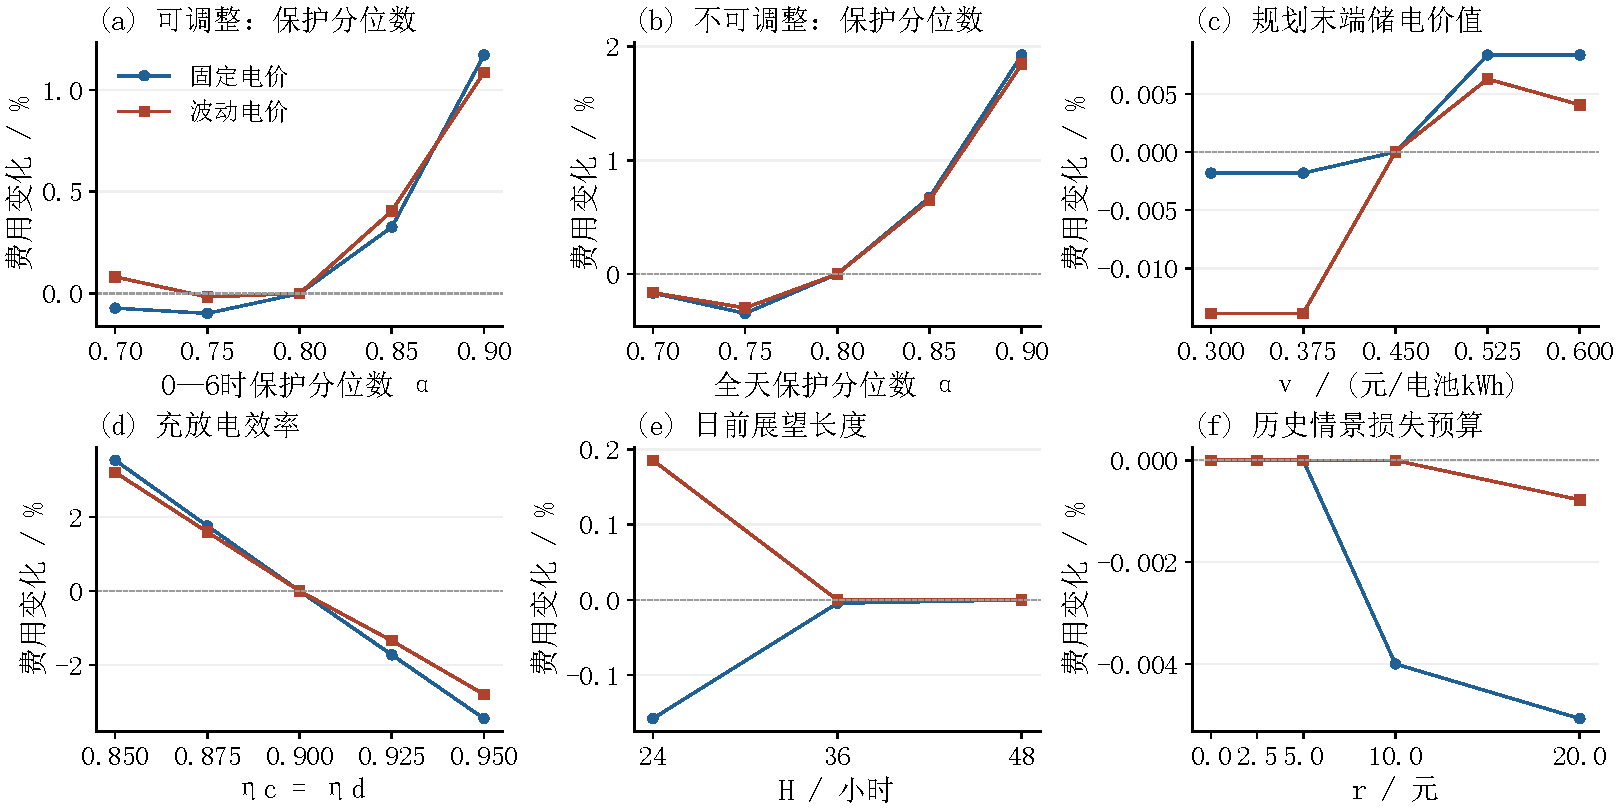
\includegraphics[width=\textwidth]{figures/统一参数敏感性.pdf}
\caption{参数变化下相对实验对照的评价期费用响应}
\label{fig:unified_sensitivity}
\end{figure}

在所设扰动范围内，效率变化引起的费用响应最大。$\eta$由0.85变为0.95时，固定电价费用相对对照$F$的变化由$+3.536\%$降至$-3.451\%$，波动电价由$+3.210\%$降至$-2.797\%$。这里改变的是单向充、放电效率，往返效率为$\eta^2$；调度与执行采用相同效率，式\eqref{eq:src41}的扣价随$\eta_d$变化。该试验表示对照配置下设备效率变化的后果，题目给定的0.90仍用于正式结果。

保护分位数在0.70至0.90内变化时，可调整方案的费用变幅为固定电价$-0.098\%$至$+1.172\%$、波动电价$-0.017\%$至$+1.086\%$；不可调整方案分别为$-0.347\%$至$+1.928\%$、$-0.299\%$至$+1.847\%$。提高保护量会同时改变正常购电和缺口补购，两类费用的平衡使响应并非处处单调。

在所取网格内，$\nu$的费用变幅绝对值不超过0.014\%，$r$不超过0.0051\%。$H$只改变日前展望，日内候选仍按最长24小时生成，情景评价仍延续至次日06:00；36小时与48小时的费用差仅为固定电价$-604.28$元、波动电价$-21.63$元。将预算$r$从5元调至20元引起的变化很小。

综上，模型在电价尺度、保护分位数、末端价值和预测展望等参数变化下均保持稳定的费用响应，说明所构建的参数体系具有良好的协调性，能够支持不同购电环境下的储能优化决策。

\subsection{年度策略局部消融检验}

为分辨各组件的作用，我们在两种电价下均使用相同负载、光伏及初始储电量6000 kWh，从1月1日连续运行365日；1月形成历史信息与储电状态，费用统一统计2--12月334日，并完成66组不同配置的消融与参数试验，重复的对照点复用同一结果。含最坏损失限制的对照$F$在固定、波动电价下的费用分别为13370019.70元和14078164.36元。正式可调整方案对应表\ref{tab:ablation}中“取消最坏损失限制”组，费用分别为13298484.49元和14018361.30元。

简单参照方案仅用历史预测，并同时取消日内调整、日前保护和规划末端价值。其余组相对$F$一次改变一项：仅0时预报组仍可在6、12、18时调整；取消日前保护组保留分位数约束候选；取消调整组保持$F$的预测和分位排程；$\nu$与$\kappa$分别取消；最坏损失组仅取消$\min_{\varsigma}\hat G_{\varsigma}\ge-r$，保留四个候选、相同历史路径及净增益均值条件。

\begingroup
\setlength{\tabcolsep}{6pt}
\Needspace{0.35\textheight}
\begin{longtable}{p{0.245\textwidth}rrrr}
\caption{组件变化相对含最坏损失限制对照$F$的费用与紧急购电量差}\label{tab:ablation}\\
\toprule
配置变化 & \multicolumn{2}{c}{费用差/元} & \multicolumn{2}{c}{紧急购电量差/kWh}\\
 & 固定电价 & 波动电价 & 固定电价 & 波动电价\\
\midrule\endfirsthead
\caption{组件变化相对含最坏损失限制对照$F$的费用与紧急购电量差（续）}\\
\toprule 配置变化 & \multicolumn{2}{c}{费用差/元} & \multicolumn{2}{c}{紧急购电量差/kWh}\\
 & 固定电价 & 波动电价 & 固定电价 & 波动电价\\
\midrule\endhead\bottomrule\endfoot
简单参照方案 & +1935181.49 & +2008272.62 & +458476.04 & +472222.26 \\
仅用0时光伏预报 & +3487.75 & +2951.83 & -930.55 & -1776.82 \\
取消日前保护量 & +268732.48 & +311355.36 & +113103.24 & +128400.37 \\
取消末端价值$\nu$ & -243.41 & -1954.81 & +40.98 & +8.82 \\
取消短缺扣价$\kappa$ & -14113.61 & -4817.05 & +191.94 & +1456.37 \\
取消最坏损失限制（正式） & -71535.21 & -59803.06 & -13861.25 & -12778.28 \\
取消日内合同调整 & +233906.53 & +269524.65 & +48720.06 & +50643.75 \\
仅用发布光伏预报 & +238475.28 & +277803.50 & +2638.32 & +5871.00 \\
\end{longtable}
\endgroup


相对$F$取消日前保护后，固定、波动电价费用分别增加2.01\%和2.21\%；光伏仅用发布预报、取消与历史预测的组合后，分别增加1.78\%和1.97\%。保持预测和保护配置，恢复$F$的日内合同调整，可使相应无调整方案的费用降低1.72\%和1.88\%。简单参照方案的费用增幅为14.47\%和14.27\%。

日内更新光伏预报后，6、12、18时各自未来6小时的合并MAE由158.13降至107.74 kW，降幅31.86\%，但费用只减少3487.75元和2951.83元，紧急电量也未同步减少。对同日费用差以7日连续移动块重采样10000次\cite{kunsch1989}，平均日差的95\%区间分别为$[-44.37,57.27]$元和$[-58.39,63.41]$元，均包含零。

末端价值的作用需结合评价边界考察。相对$F$取消$\nu$后，账单分别减少243.41元和1954.81元；另以统一参考价0.45元/电池kWh计算$C_{\rm ref}=C-0.45(E_{\text{末}}-E_{\text{初}})$，两组相对$F$仅差$+78.24$元和$-12.49$元。相对$F$取消$\kappa$后费用下降，但紧急购电量增加，调整次数由65、77次增至296、261次；两组平均日费用差区间分别为$[-67.95,-16.14]$元和$[-35.52,13.65]$元。短缺扣价在含最坏损失限制的配置下减少了合同变动；固定电价下有费用代价，波动电价下费用差方向尚不稳定。

取消最坏情景限制后，固定、波动电价费用分别减少71535.21元和59803.06元，11个月费用均下降；日费用与日紧急电量的最大值及95\%分位数也均下降。相应平均日费用差的95\%区间为$[-303.52,-130.51]$元、$[-274.80,-97.25]$元。

波动电价下，取消周同期偏差校正后，日前电价MAE由0.04803降至0.04715元/kWh；不可调整方案费用减少3288.75元，含最坏损失限制的可调整组相对$F$增加7980.31元。两者平均日差区间分别为$[-31.06,10.57]$元和$[-20.53,87.38]$元。

综合消融结果，净负荷保护、组合预测和日内合同调整共同改善了购电费用与紧急购电控制效果，完整模型在固定电价和波动电价场景下均取得稳定的综合收益，体现了各模块协同集成的优势。

\subsection{滚动预测起点与分月稳定性检验}
对每个预测起点$d$，我们仅使用该起点预测的未来一天进行误差统计，并将48096个10分钟目标时段按月份分组，定义
\begin{equation}\label{eq:validation_metrics}
\begin{aligned}
\mathrm{MAE}&=\frac1n\sum_i|y_i-\hat y_i|,\qquad
\mathrm{RMSE}=\sqrt{\frac1n\sum_i(y_i-\hat y_i)^2},\\
\mathrm{WAPE}&=\frac{\sum_i|y_i-\hat y_i|}{\sum_i|y_i|}\times100\%,\qquad
S_m=\frac{C_m^{\mathrm{base}}-C_m^{\mathrm{roll}}}{C_m^{\mathrm{base}}}\times100\%.
\end{aligned}
\end{equation}
其中$n$为评价时段数，$S_m$为第$m$月正式可调整方案相对对应日前方案的费用节省率。WAPE采用全样本实际值总量作分母，适合包含零出力时段的光伏序列。模型参数固定为正式配置，滚动更新的对象为历史误差及预测校正量。

\Needspace{0.35\textheight}
\begin{longtable}{rrrrrr}
\caption{分月预测误差与正式方案费用节省率}\label{tab:monthly_stability}\\
\toprule 月份 & 时段数 & 光伏MAE/kW & 电价MAE/(元/kWh) & 固定价$S_m$/\% & 波动价$S_m$/\%\\\midrule\endfirsthead
\caption{分月预测误差与正式方案费用节省率（续）}\\\toprule 月份 & 时段数 & 光伏MAE/kW & 电价MAE/(元/kWh) & 固定价$S_m$/\% & 波动价$S_m$/\%\\\midrule\endhead\bottomrule\endfoot
2 & 4032 & 99.59 & 0.04703 & 1.54 & 1.48\\
3 & 4464 & 128.04 & 0.04250 & 3.45 & 3.40\\
4 & 4320 & 155.15 & 0.04331 & 6.63 & 6.26\\
5 & 4464 & 145.25 & 0.04690 & 4.00 & 3.45\\
6 & 4320 & 143.50 & 0.05406 & 8.21 & 8.51\\
7 & 4464 & 154.09 & 0.05690 & 2.69 & 2.90\\
8 & 4464 & 154.21 & 0.04807 & 4.00 & 3.35\\
9 & 4320 & 134.08 & 0.05917 & 5.21 & 4.89\\
10 & 4464 & 137.59 & 0.04294 & 2.29 & 2.10\\
11 & 4320 & 78.41 & 0.03883 & 0.94 & 1.19\\
12 & 4464 & 74.27 & 0.04869 & 1.35 & 1.85\\

\end{longtable}
两类正式可调整方案在11个月的费用均低于对应日前方案，6月降幅最大，分别为8.21\%和8.51\%；11月最小，分别为0.94\%和1.19\%。

